\documentclass{beamer}
\usetheme{Copenhagen}

\usepackage{siunitx}
\newcommand{\h}{\unit{\hour}}
\newcommand{\ph}{\unit{\per\hour}}
\newcommand{\um}{\unit{\micro\metre}}
\newcommand{\pums}{\unit{\per\micro\metre\squared}}
\newcommand{\nm}{\unit{\nano\mole\per\litre}}

\usepackage{amsmath}
\usepackage{amssymb}
\usepackage{cancel}
\usepackage{graphicx}
\graphicspath{{../images/}}

\title{An ODE Model of CLASP Mutants in \emph{A. Thaliana}}
\author{Riley Wheadon}
\institute{University of British Columbia}

\begin{document}

\begin{frame}
\frametitle{Complete Signalling Network}
\begin{figure}
  \centering
  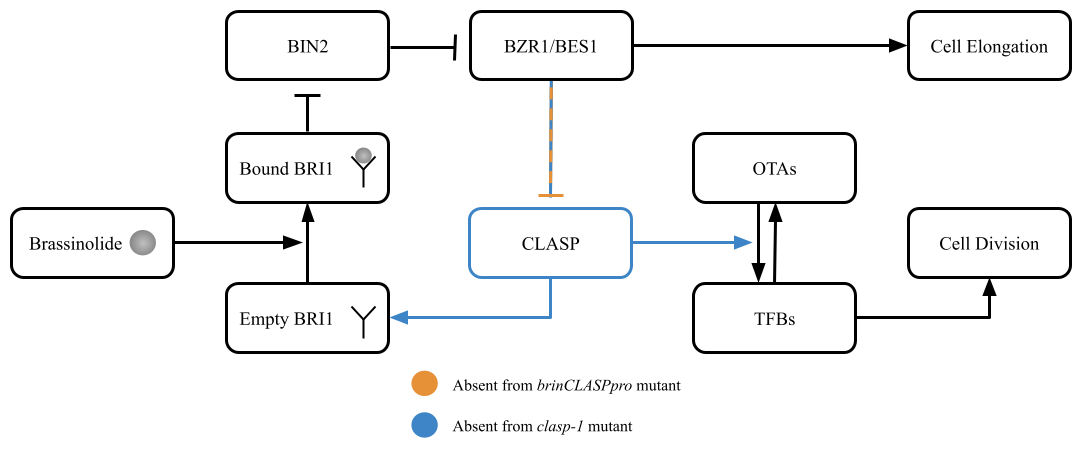
\includegraphics[width=\textwidth]{network-complete.png}
  \caption{The signalling network used to inform model development.}
\end{figure}
\end{frame}

\begin{frame}
\frametitle{Simplified Signalling Network}
\begin{figure}
  \centering
  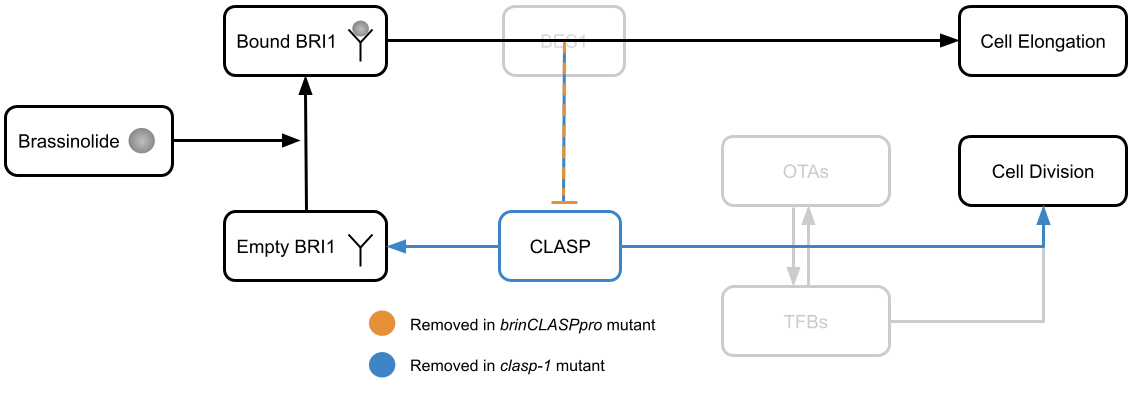
\includegraphics[width=\textwidth]{network-simplified.png}
  \caption{The abridged signalling network used in the model itself.}
\end{figure}
\end{frame}

\begin{frame}
\frametitle{Cell Division Model}
\begin{figure}
  \centering
  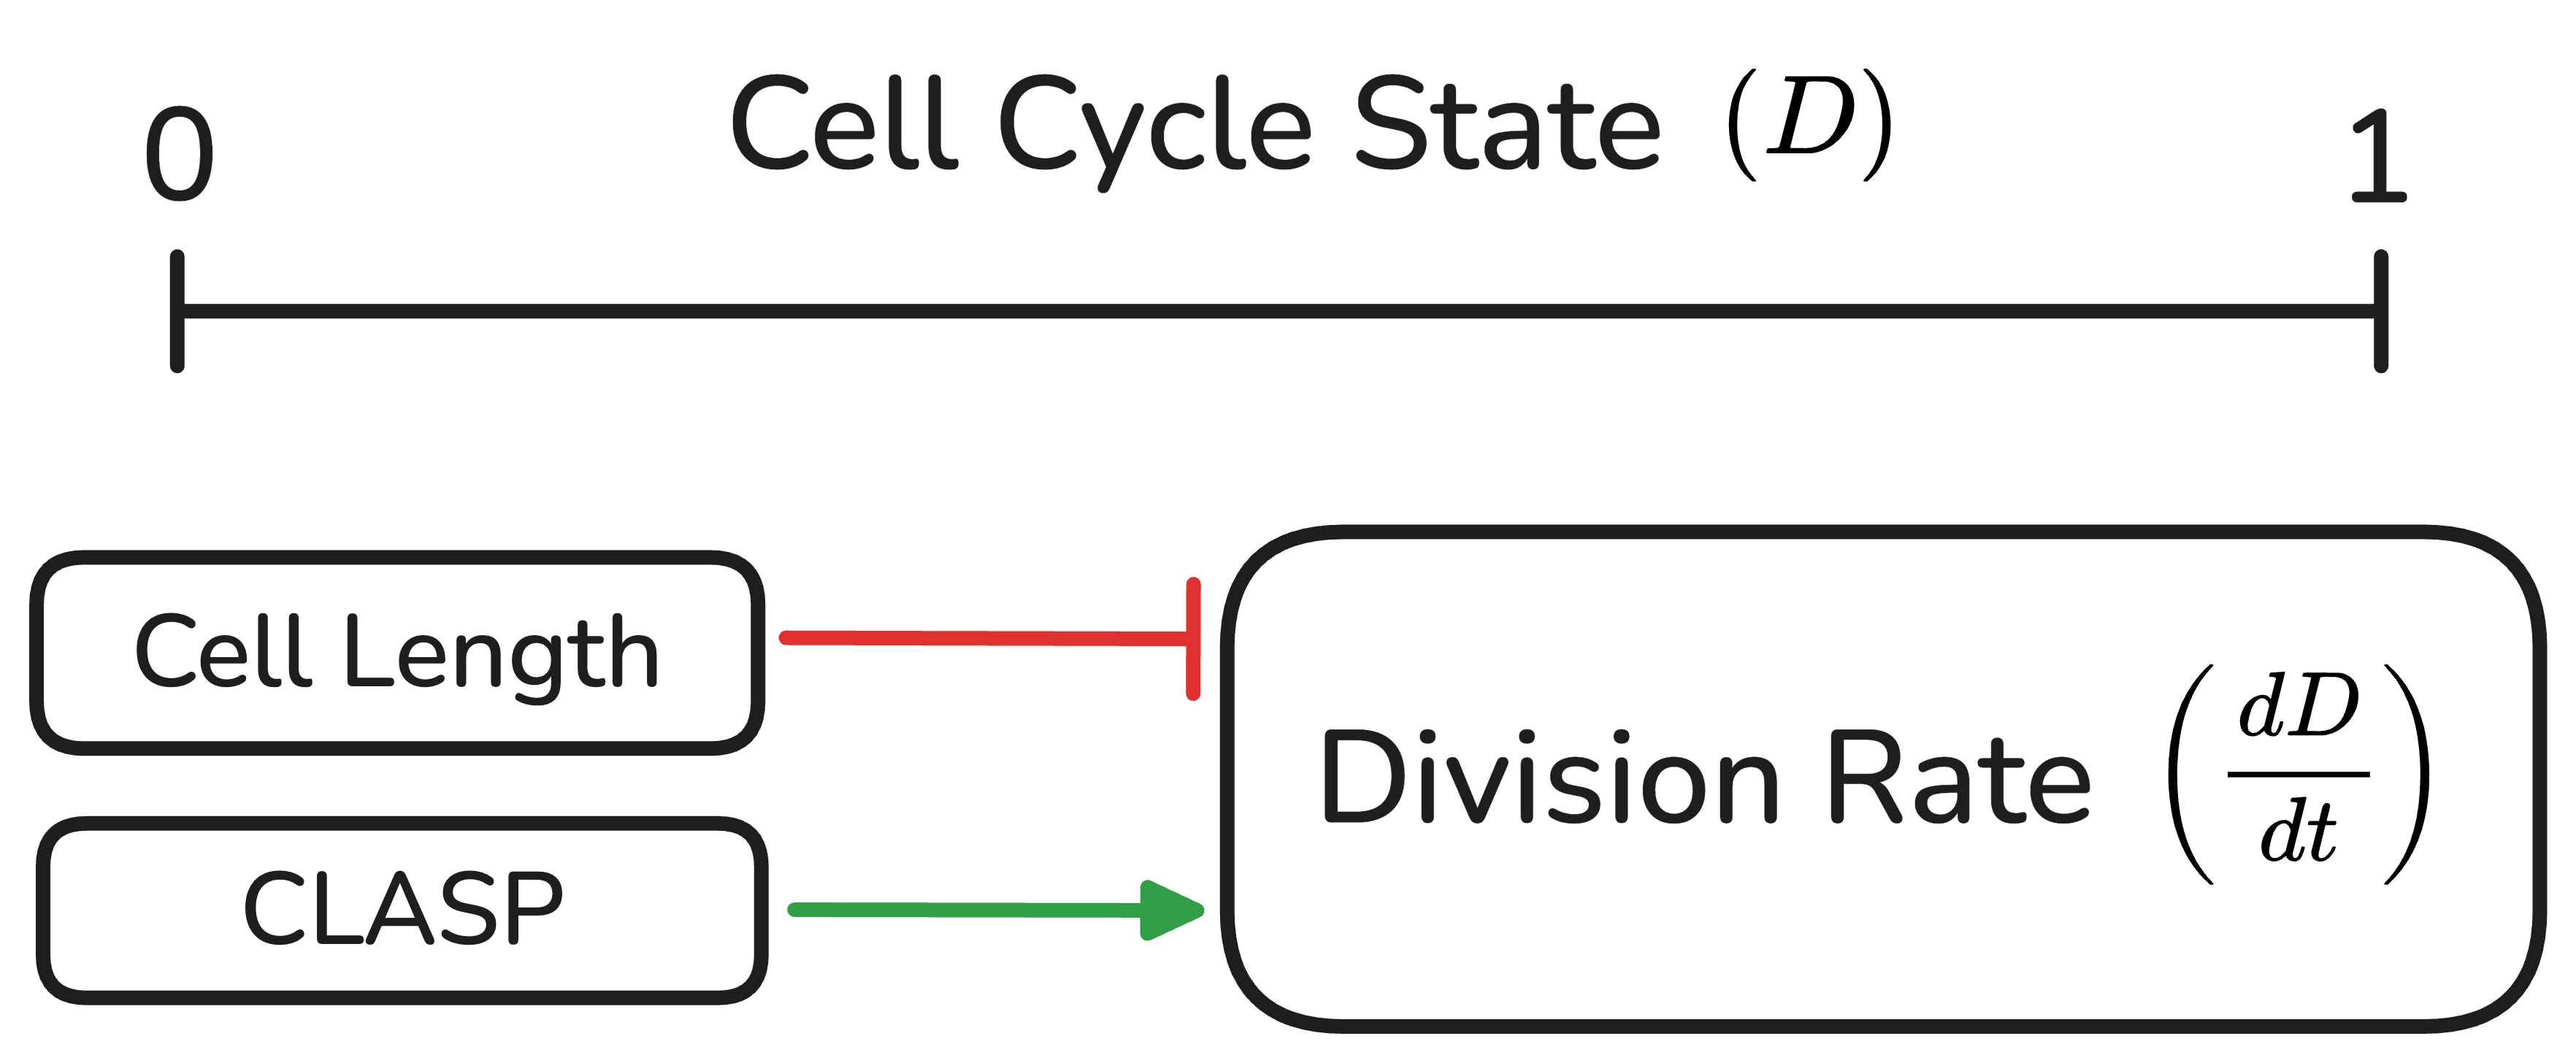
\includegraphics[width=\textwidth]{division-model.png}
  \caption{Overview of the cell division model.}
\end{figure}
\end{frame}

\begin{frame}
\frametitle{Data Preparation}
\begin{figure}
  \centering
  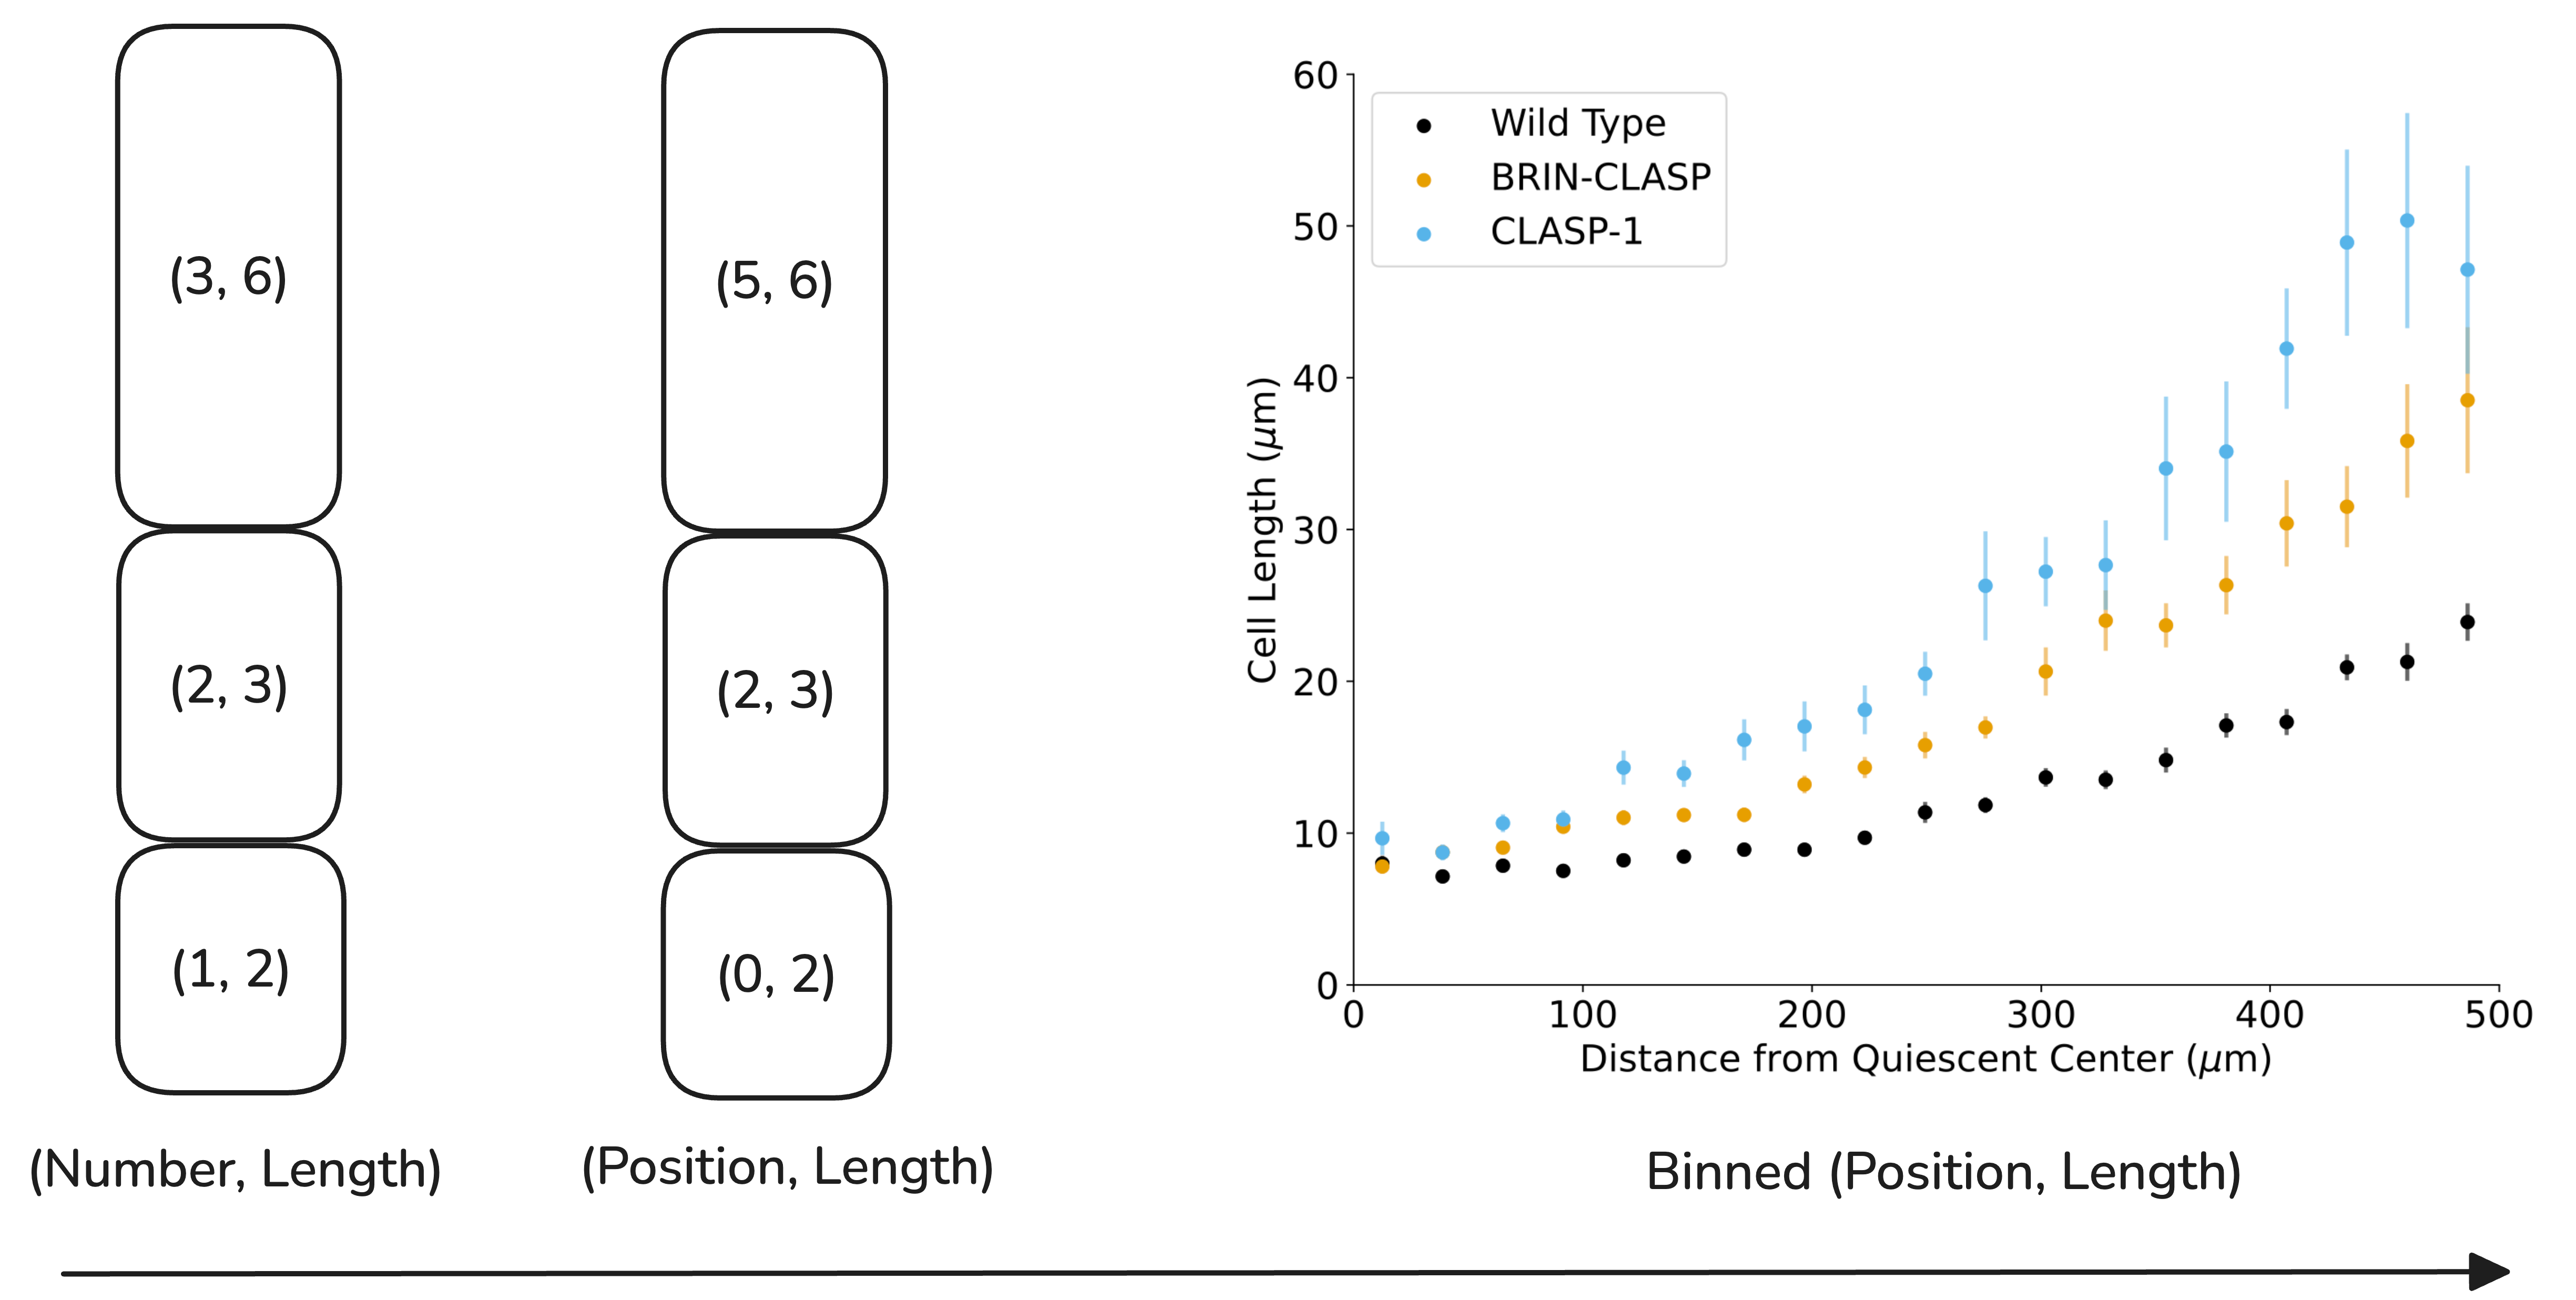
\includegraphics[width=\textwidth]{data-processing.png}
  \caption{Overview of the data processing pipeline.}
\end{figure}
\end{frame}

\begin{frame}
\frametitle{Initial Results (1/2)}
\begin{figure}
  \centering
  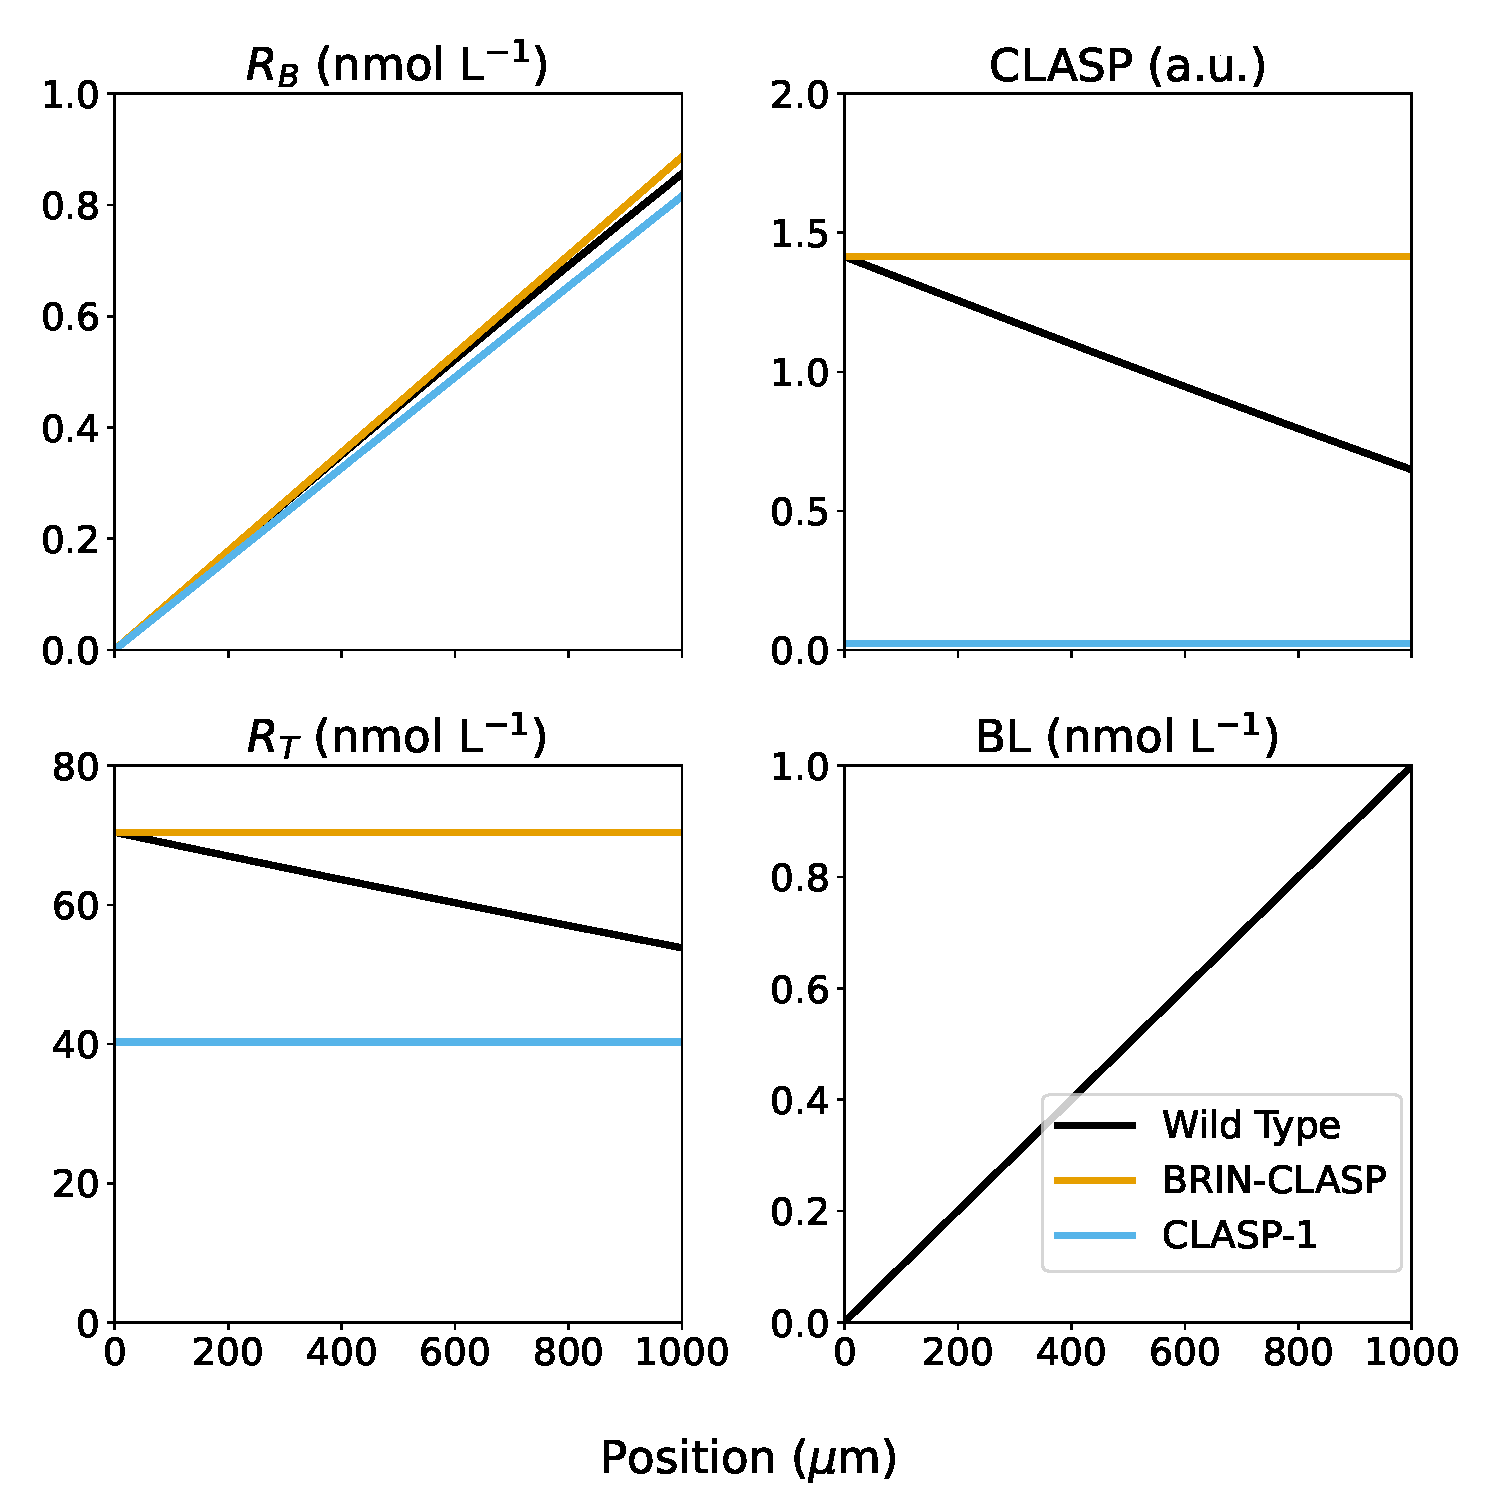
\includegraphics[height=16em]{bes1-mutants.pdf}
  \caption{Estimated protein levels from the intracellular model.}
\end{figure}
\end{frame}

\begin{frame}
\frametitle{Initial Results (2/2)}
\begin{figure}
  \centering
  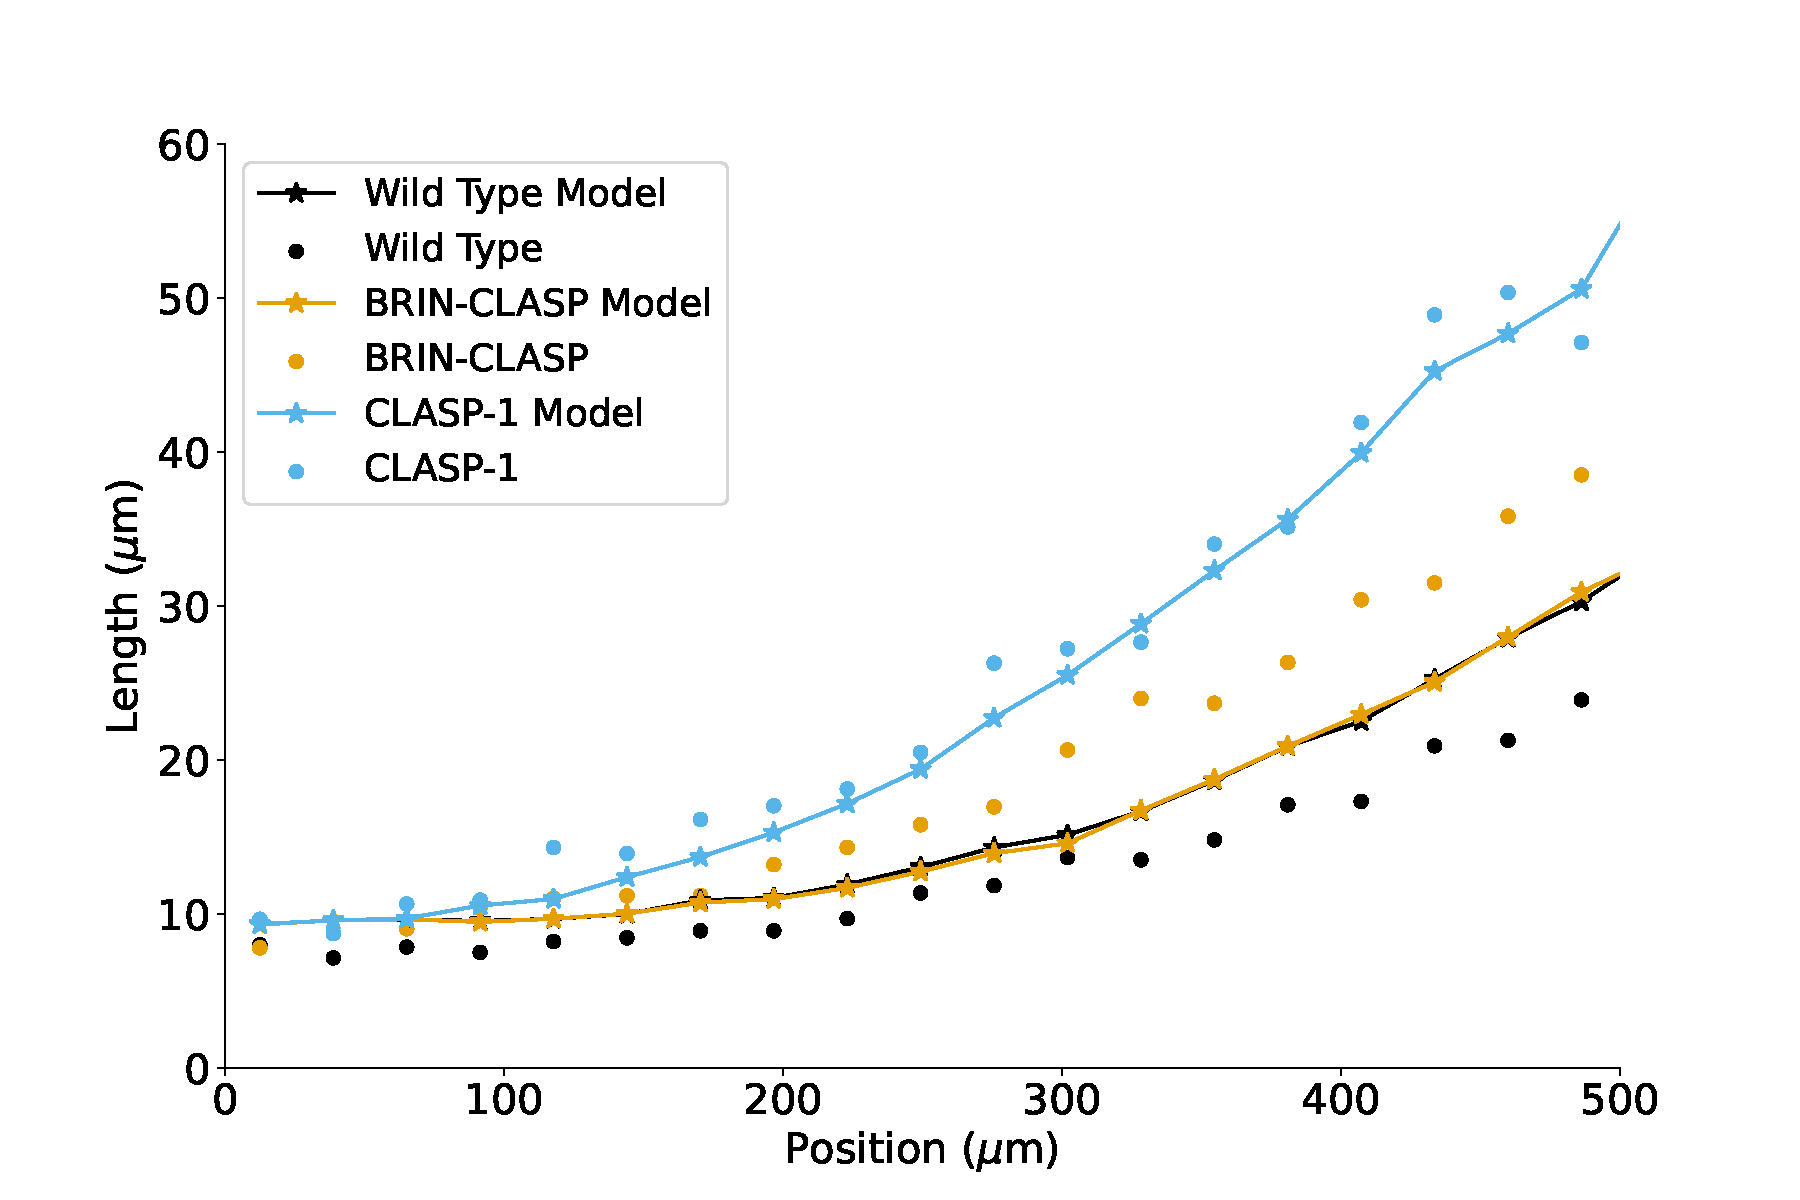
\includegraphics[height=16em]{column-original-fit.pdf}
  \caption{The initial model was unable to explain \emph{brinCLASPpro}.}
\end{figure}
\end{frame}

\begin{frame}
\frametitle{Explaining \emph{brinCLASPpro}}
\begin{columns}
  \begin{column}{0.5\textwidth}
    Idea 1: Increasing Growth
    \begin{itemize}
      \item Decrease $R_{T}$ or increase $B$ relative to the wild type.
      \item Additional growth needs to occur in the division zone.
    \end{itemize}
    \bigskip
    \emph{This didn't work...}
  \end{column}
  \begin{column}{0.5\textwidth}
    Idea 2: Inhibiting Division
    \begin{itemize}
      \item Decrease cell division relative to the wild type. 
      \item This may be caused by an excess of CLASP.
    \end{itemize}
    \bigskip
    \emph{This did work!}
  \end{column}
\end{columns}
\end{frame}

\begin{frame}
\frametitle{Improved Results (1/3)}
\begin{figure}
  \centering
  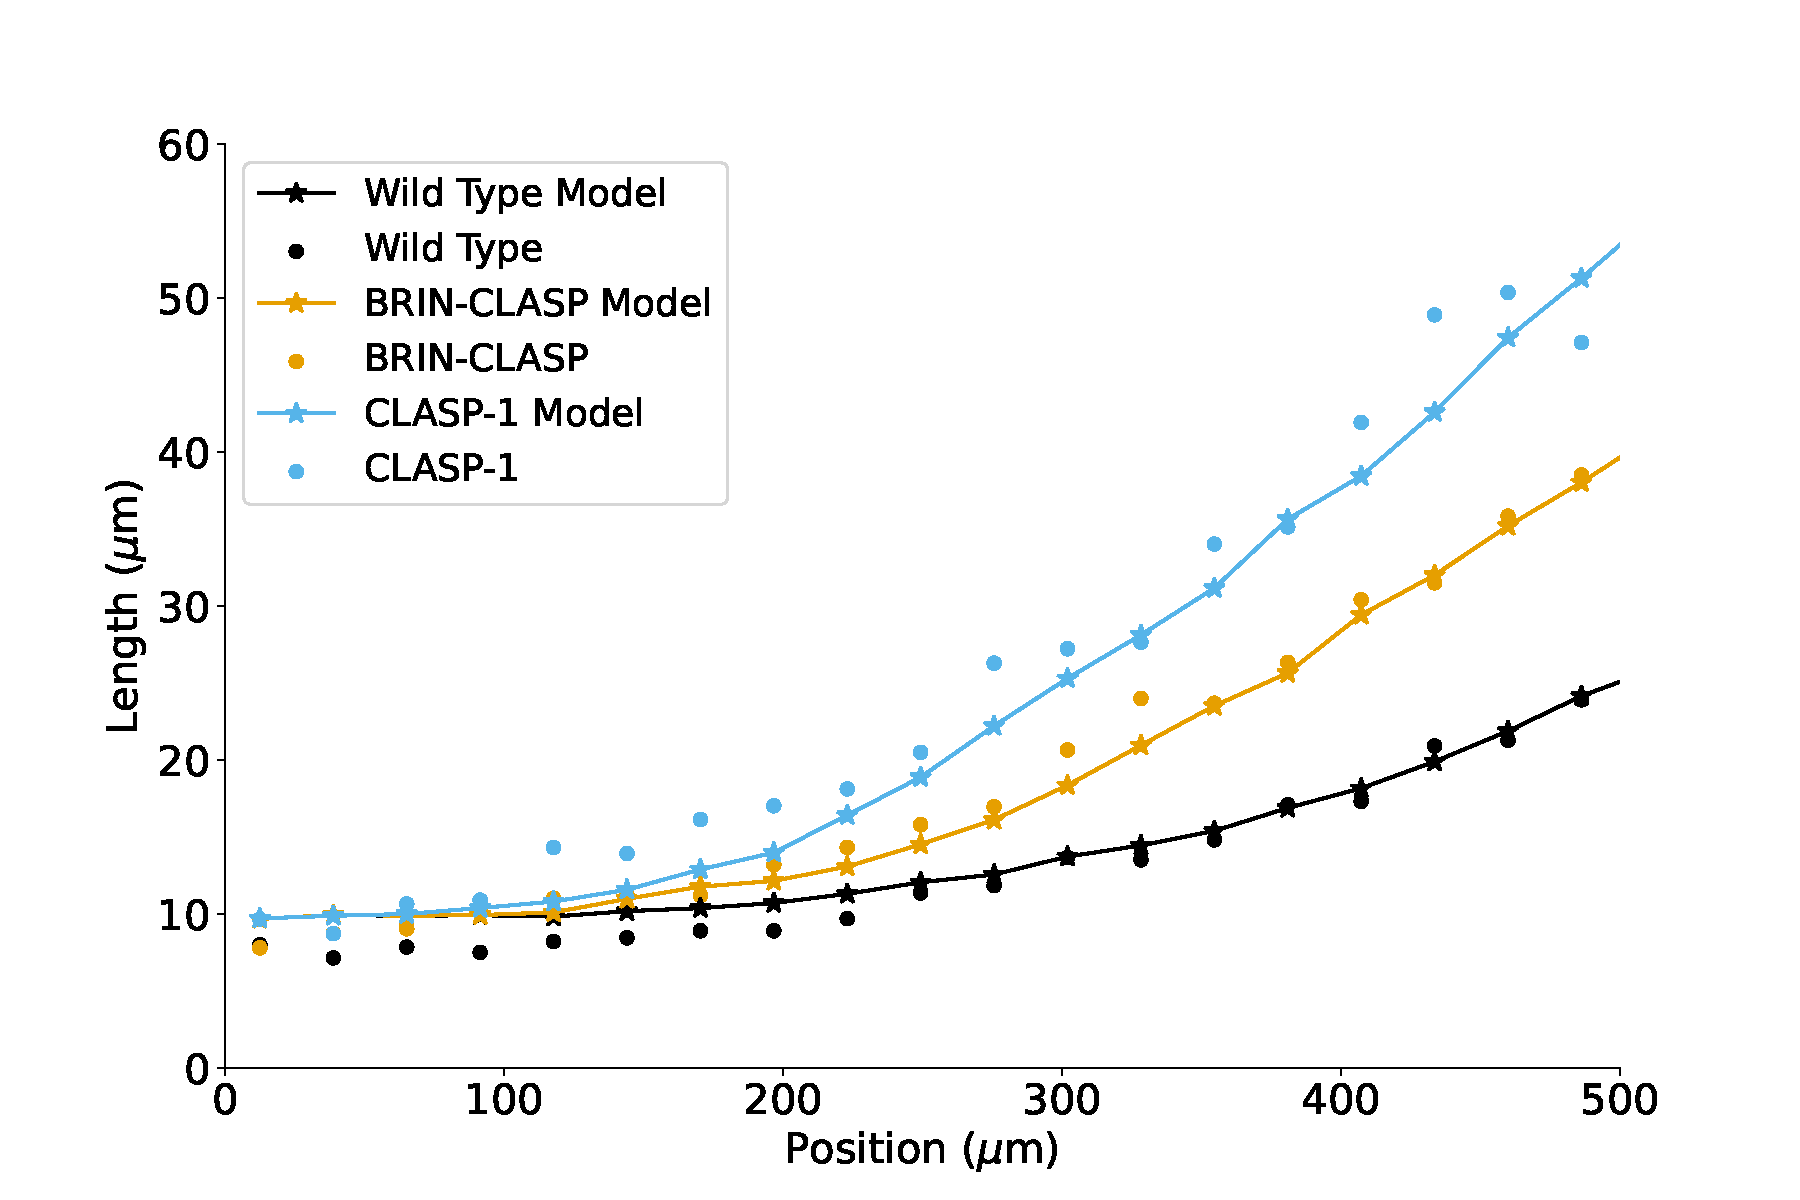
\includegraphics[height=16em]{column-modified-fit.pdf}
  \caption{Inhibition of cell division by high concentrations of  CLASP is sufficient to differentiate the \emph{brinCLASPpro} mutant from the wild type.}
\end{figure}
\end{frame}

\begin{frame}
\frametitle{Imrpoved Results (2/3)}
\begin{figure}
  \centering
  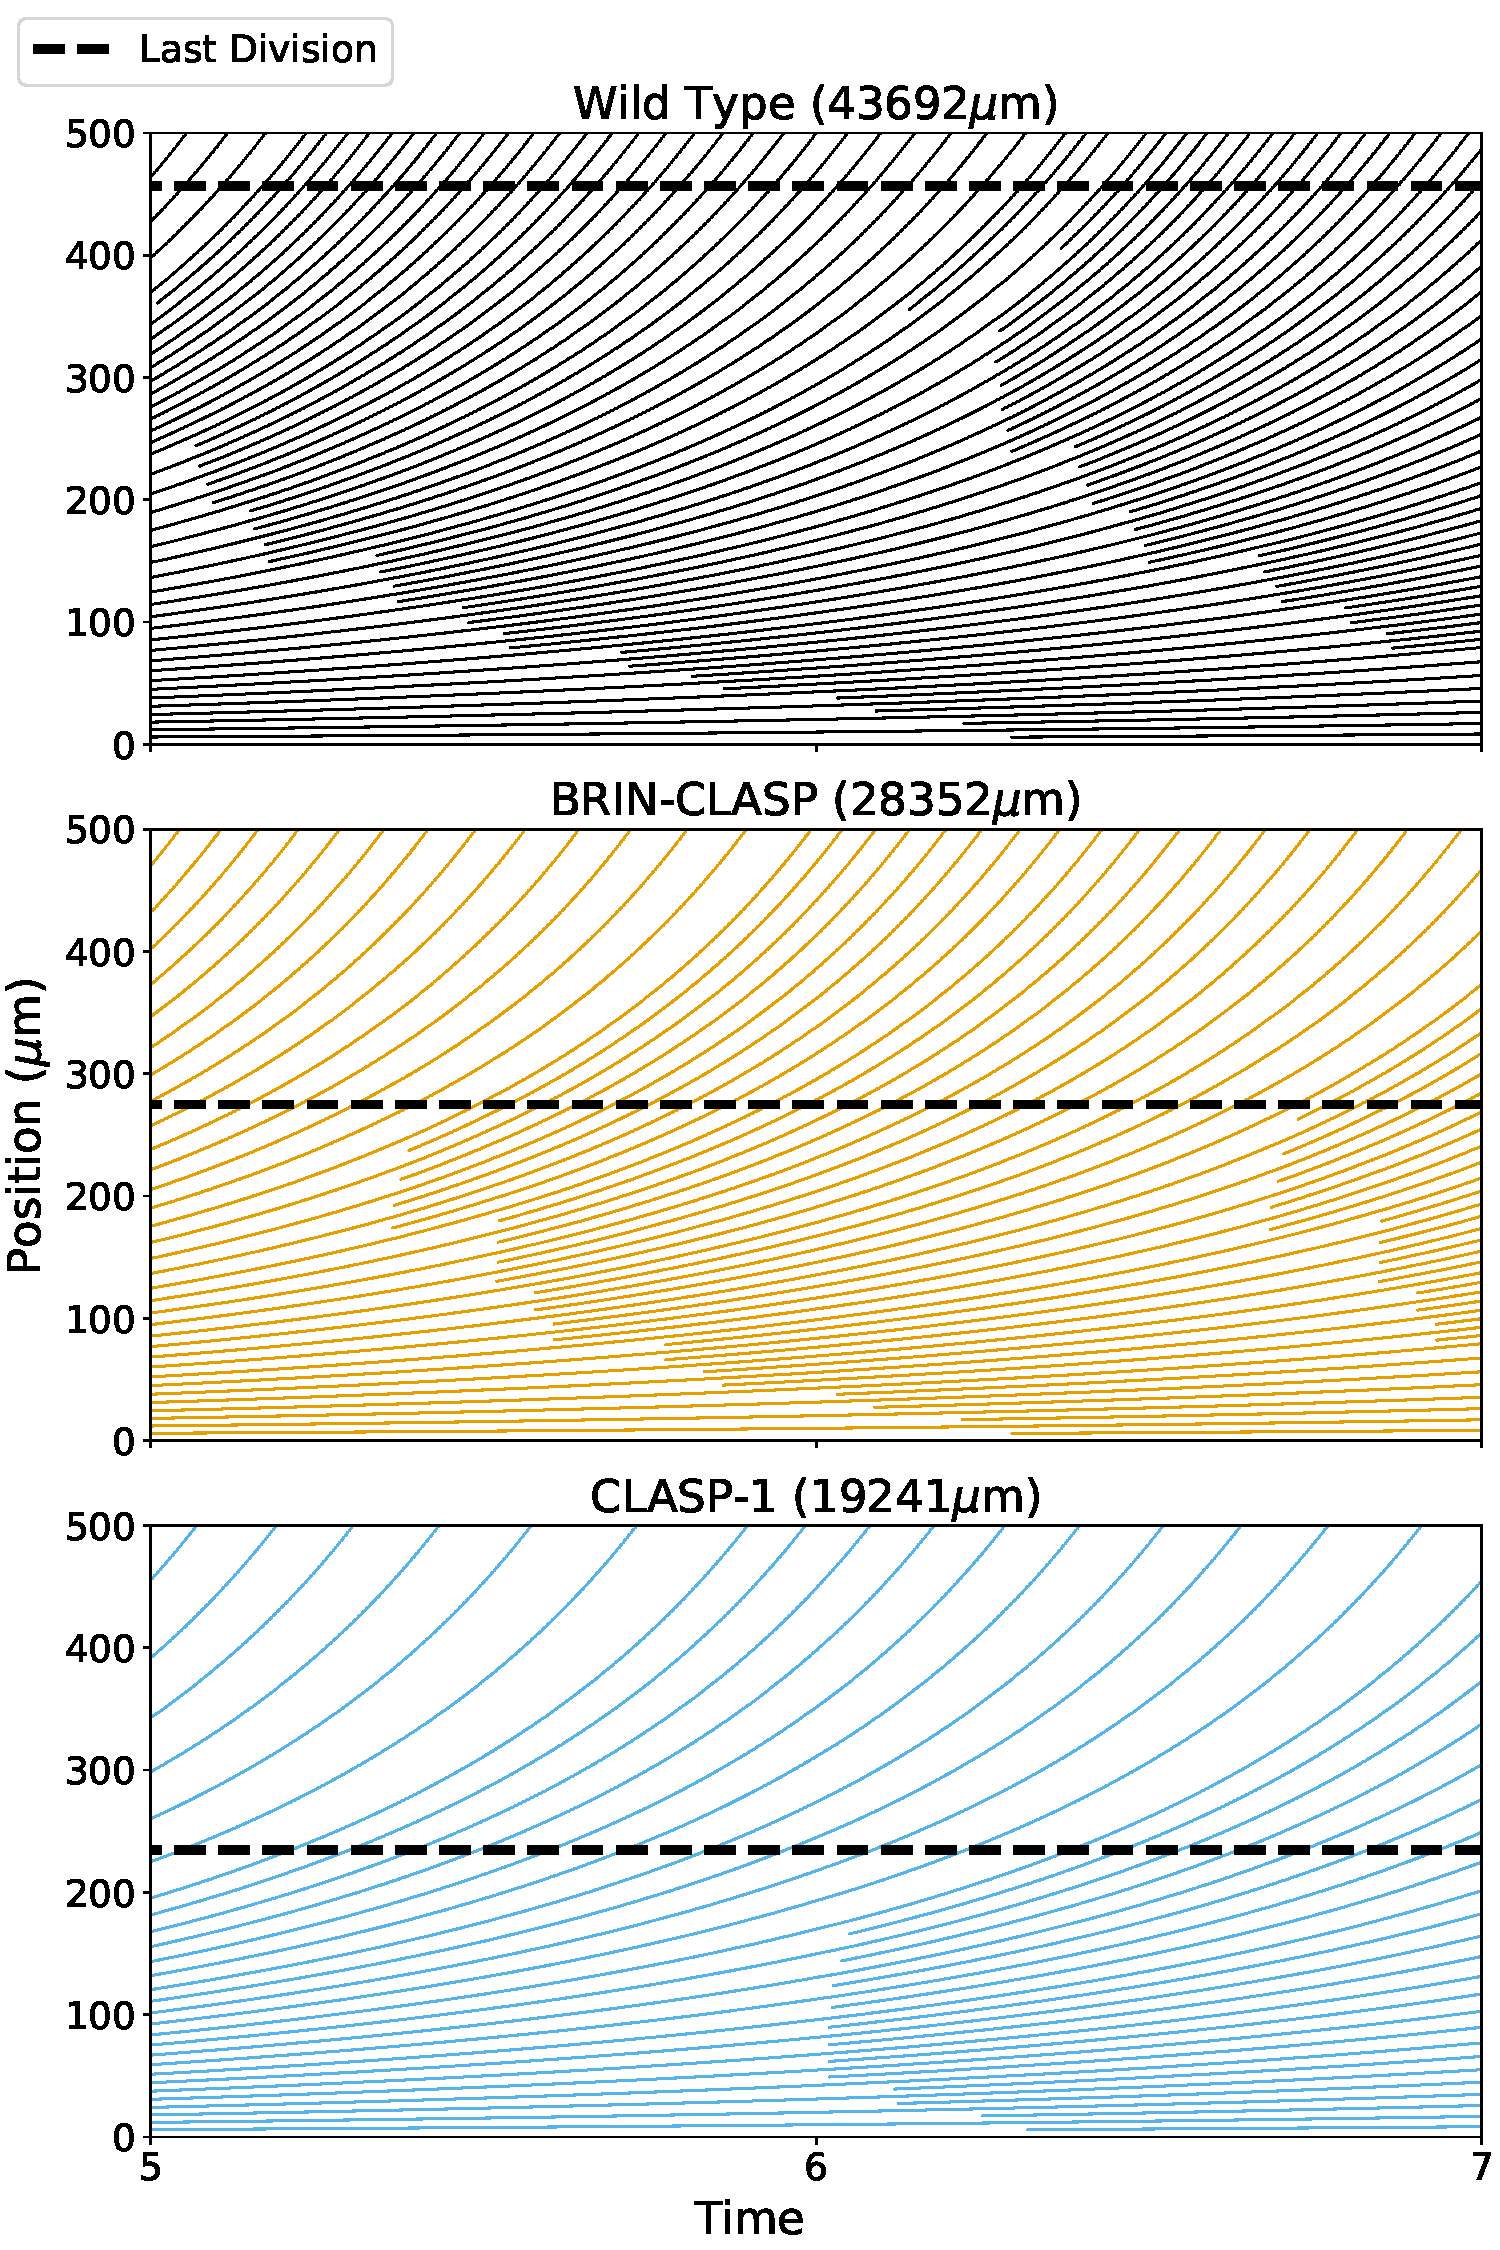
\includegraphics[height=16em]{column-modified-profile.pdf}
  \caption{Division zone profiles for each mutant.}
\end{figure}
\end{frame}

\begin{frame}
\frametitle{Improved Results (3/3)}
\begin{figure}
  \centering
  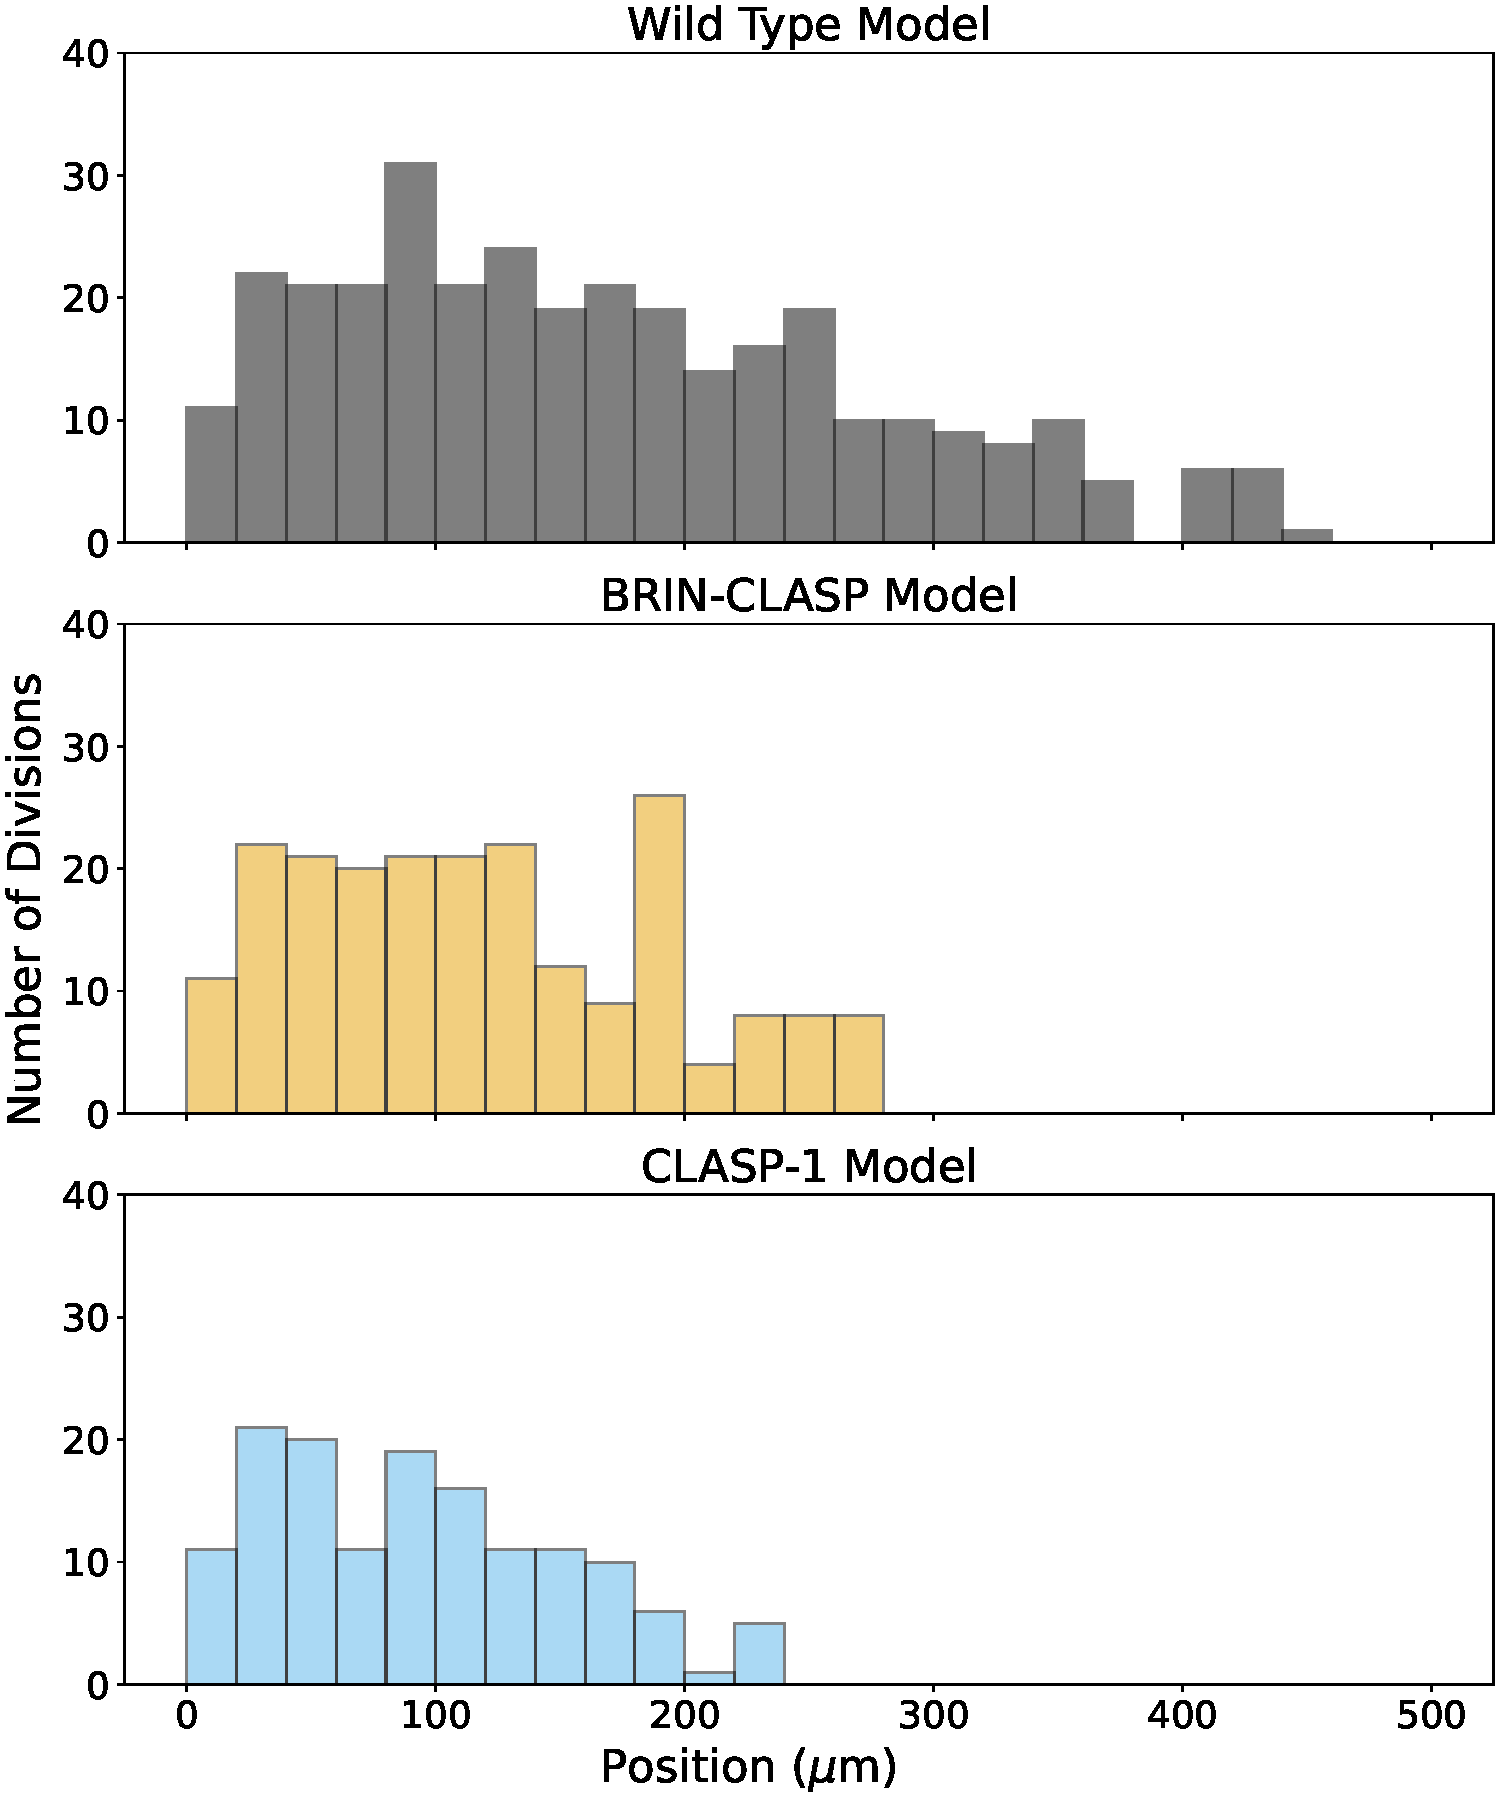
\includegraphics[height=16em]{column-modified-histogram.pdf}
  \caption{Histogram of division locations by mutant.}
\end{figure}
\end{frame}
\end{document}


